\newpage\section{Sistema D – Sistema de Segurança}


\begin{figure}[H]
    \centering
    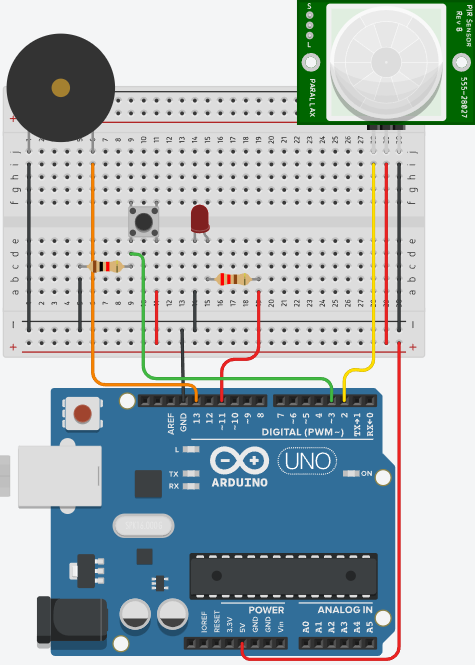
\includegraphics[scale=0.6,angle=-90]{images/hardware/sisD_tinkercad.png}
    \selectlanguage{portuguese}\caption{Esquema do Sistema}
\end{figure}

\begin{table}[H]
    \centering
    \setlength{\arrayrulewidth}{0.5mm}
    \renewcommand{\arraystretch}{1.5}
    \begin{tabular}{|l|c|}
        \hline
        \multicolumn{1}{|c|}{Componentes} & \multicolumn{1}{|c|}{Quantidade}\\ [0.8ex] 
        \hline
        Arduino & 1x\\
        \hline
        LED Vermelho & 1x\\
        \hline
        Alarme Sonoro & 1x\\
        \hline
        Botão & 1x\\
        \hline
        Resistência 220$\Omega$ & 1x\\
        \hline
        Resistência 1k$\Omega$ & 1x\\
        \hline
    \end{tabular}
    \selectlanguage{portuguese}
    \caption{Lista dos Componentes}
\end{table}

O botão encontra-se ligado à porta digital n$^{o}$ 3.

O sensor PIR está ligado à porta digital n$^{o}$2.

O LED Vermelho encontra-se ligado à porta analógica n$^{o}$1.

As portas 2 e 3 apresentam capacidade de Interrupt.